\subsection{External Clock and Pull Model}

The overarching design principle of Databus is that it is simply a lossless transporter of changes that have been committed upstream. Each change set is annotated with a monotonically increasing system change number~(SCN). This number is assigned by the data source and typically system specific. For example, Oracle attaches an SCN to each commit, while MySQL's commits can be identified uniquely through their offset in the binary log (binlog). As these changes flow through the ecosystem, derived state gets created by consumers and is associated back to the change stream through this number. This is important not just for auditing, but also to recover from failures and resume processing without missing any changes.  The system therefore is externally clocked. All parts of the Databus infrastructure track the lineage of data records and the progress of consumers using only the SCN of the external system. Physical offsets are only used as optimizations in internal transport but are never used as source of truth. 

There are many advantages of favoring pull over push in this particular context. We need to support a large number of consumers and allow them to consume from any arbitrary point in time. The most natural place to keep state of how much of the SCN timeline has been really processed is the consumer, because that is where the processing is taking place. Keeping state at the consumer naturally leads to a pull-based data transfer model. 
%The requirement to support change data consumption from an arbitrary point in the change timeline naturally leads to a pull data transfer model for consumers. 
The process can be entirely governed by the consumers; at any moment, they may decide to rollback to a previous point. 
Thus, all Databus components have to be stateless. 

Further, the requirements for not introducing new points of failures and source consistency preservation led us to adopt a pull data transfer model for the DB fetcher. In a hypothetical push-based model, failures in pushing the changes from the DB fetcher to the relay will either lead to aborted transactions (violating the first requirement) or changes that are lost by Databus (violating the second requirement). 

Figure~\ref{fig:pull-model} shows the interactions between the different fetcher components and the source clock across the relay, bootstrap log and snapshot store. In this example, the source has generated changes until SCN 102400, the relay has an in-memory buffer that covers all changes from 70000 to 100000, the bootstrap service's persistent log covers all changes from 30000 to 90000, and the bootstrap service's snapshot store covers all changes from 0 to 80000. Depending on where the consumer is currently at, it will pull from either the relay or the bootstrap service. 

\begin{figure}
\centering
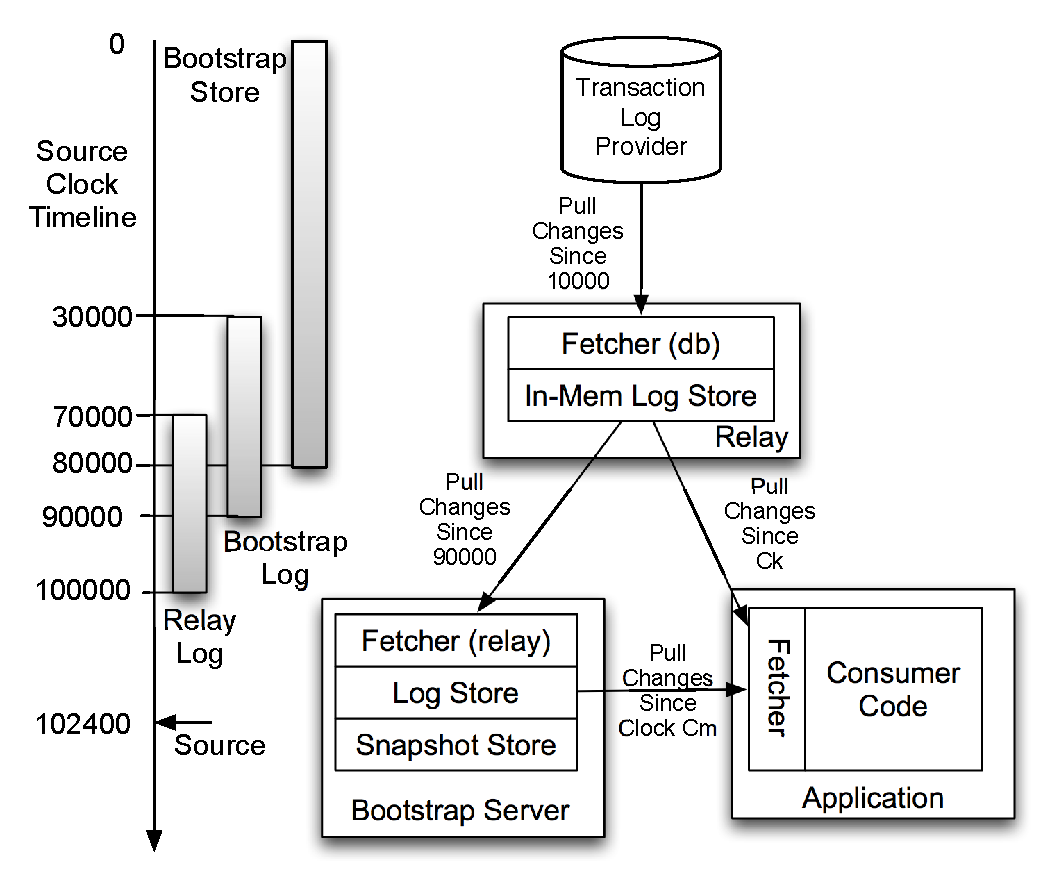
\epsfig{file=figures/databus-pull-model.eps, scale=0.50}
\caption{Pull Model and Source Clock}
\label{fig:pull-model}
\end{figure}

In addition to supporting simple restart and recovery semantics, this design also makes it very easy to integrate with non-Databus based data flows. 
%This is a very important design decision because it allows very simple restart and recovery semantics as well as integration with non-Databus based data flows. 
For example, an application can take a dump of an Oracle database, perform arbitrary processing on that dump, and then seamlessly tap into the Databus stream to get all changes that have happened to the database without missing a single change. The only requirement is that the original Oracle dump should be stamped with the same clock (Oracle's SCN system) that the Oracle Databus fetcher uses to pull changes out from Oracle. 

\subsection{Source Data Extract}
%The Fetcher: External Clock and Pull model}

Databus has been designed to support extraction from different data sources. This flexibility is achieved by allowing different fetchers to be developed and plugged into the pipeline. 
The fetcher is typically an embedded thread that gets run from within a relay and must follow a few semantic constraints.
As described above, each change set must be annotated with a monotonically increasing clock value that we refer to as the system change number~(SCN) of the change set.
This mapping from change set to SCN is immutable and assigned at commit time by the data source, therefore Databus can run multiple independent fetchers following the same timeline of changes without any need for synchronization. 
The fetcher is initialized with an SCN on startup, and must start pulling changes that are newer than this SCN from the data source. This in turn adds a ``rewindability'' requirement on the data source. 
The data source must be able to keep enough history in its change log or the fetcher must be written in a way that supports going back to pull from an arbitrary point in time. 
In practice, this requirement does not add any extra complexity on the source, but depending on the implementation, it can have a performance impact on the online writes that are happening on the data store. 
% as long as this lookback window is bounded (within a day or two). 
The way the Oracle fetcher is written, it can go back all the way to time zero, but since it queries the in-database tables, these queries get progressively expensive and impact the OLTP workload on the system. 
The MySQL fetcher mines the binary log directly, and can therefore rewind back to as much time as the storage on the MySQL machine will allow to retain without any performance penalty on the OLTP workload. 
We talk in detail about the implementation of these two fetchers in Section~\ref{sec:Implementation}.
Overall, this centralization of complexity onto the fetcher component leads to very simple persistence and failure-recovery protocols downstream. 
At the same time, fault-tolerance and high-availability in the relay tier and the presence of the snapshot store reduces the likelihood of having to go back in time on the data source, thus keeping the fetcher overhead low. 

%Extractors keep track of where they are in the timeline using checkpoints which typically contain a highwatermark corresponding to the contiguous section of the timeline that has been reliably processed so far. The fetcher is expected to be initialized with a checkpoint when it starts up or recovers from a failure. Once initialized, the fetcher keeps pulling changes from the data-source from that checkpoint onwards. As changes get processed, the fetcher keeps advancing the highwatermark and periodically stores the checkpoint in some persistence layer. This pure pull model ensures that the Databus transport layer is lossless. The only guarantees needed from the persistence layer is to not lose changes out of order. 

%Similarly, the only requirement this adds on the data source is that it should be able to support rewindable consumption; the fetcher can sometimes go back in time on failures. In most of the systems we've seen, this requirement does not add extra complexity on the source as long as this lookback window is bounded (within a day or two). The way the Oracle fetcher is written, it can go back all the way to time zero, but at the cost of queries that get progressively expensive. The MySQL fetcher can rewind back to as much time as the storage on the MySQL machine will allow to retain, without any performance penalties. This centralization of complexity onto the fetcher component leads to very simple persistence and failure-recovery protocols downstream.
